\documentclass[a4paper,11pt,dvipdfmx]{ujarticle}
% パッケージ
\usepackage{graphicx}
\usepackage{url}
% レイアウト指定を記述したファイルの読み込み
\input{layout}

% タイトルと氏名を変更せよ.
\title{日本におけるデジタル化の状況}
\author{G584332025 川畑 皓夜}

\begin{document}

\maketitle %ここにタイトルが入る
\section{デジタル競争力ランキング}
国際経営開発研究所(IMD)の調査\cite{IMD}によると、
日本のデジタル競争力のランキングは図\ref{fig:ランキング}
に示すように、調査対象の64カ国中、総合で28位、知識分野で25位となっている。


% ここから本文
% 節見出し: \section{}
% を使う

% 本文(1)
%  参考文献の参照: \cite{}
%  図番号の参照: \ref{}
% を使う
% 文献データベースのキーワードは oecd と imd
% になっている.

% 図の挿入
\begin{figure}[htbp]
    \centering
    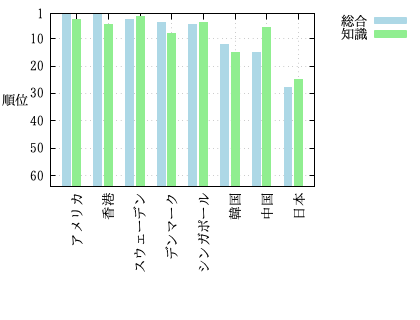
\includegraphics[width=0.7\linewidth]{fig31.png}
    \caption{デジタル競争力ランキング(64カ国中)}\label{fig:ランキング}
 \end{figure}
% で囲み

\section{ブロードバンドの整備状況}
OECDによるブロードバンド回線の普及に関する調査\cite{OECD}によると、
表\ref{tbl:モバイルブロードバンドの加入者数(100人あたり)}に示すように、日本における100人あたりのモバイルブロードバンドの加入者数は190.5で、第1位になっている。2位はエストニアで、3位米国と続く。

% 本文(2)


 \begin{table}[htbp]
    \caption{モバイルブロードバンドの加入者数(100人あたり)}
    \centering
    \label{tbl:モバイルブロードバンドの加入者数(100人あたり)}

    \begin{tabular}{|c|l|r|}\hline
        順位 & 国名 & 加入者数 \\
        \hline
        1位 & 日本 & 190.5  \\
        \hline
        2位 & エストニア & 179.9 \\
        \hline
        3位 & 米国 & 169.0 \\
        \hline
        4位 & フィンランド & 157.0 \\
        \hline
        5位 & デンマーク & 141.7 \\
        \hline
        6位 & ラドビア & 141.6 \\
        \hline
        7位 & イスラエル & 139.9 \\
        \hline 
        8位 & オランダ & 133.7 \\
        \hline
        9位 & ポーランド & 131.3 \\
        \hline
        10位 & スウェーデン & 127.2 \\
        \hline
    \end{tabular}   
\end{table} 
% ーーー
% 見出し(3)
% 考察
\section{考察}
 \begin{itemize}
    \item 日本がデジタル競争力が低い要因として「紙文化」や「ハンコ文化」などの変化を嫌う文化的な壁がある。
    \item 日本がブロードバンド整備状況が高い理由として、世界トップレベルの光ファイバー普及率や人口密度の高さによる都市部への集中設備が挙げられる。
 \end{itemize}
 
% を使って箇条書きで記述する

% ここに参考文献が入る
%
\bibliographystyle{junsrt}
\bibliography{exercise.bib}

\end{document}